% This is "sig-alternate.tex" V2.1 April 2013
% This file should be compiled with V2.5 of "sig-alternate.cls" May 2012
%
% This example file demonstrates the use of the 'sig-alternate.cls'
% V2.5 LaTeX2e document class file. It is for those submitting
% articles to ACM Conference Proceedings WHO DO NOT WISH TO
% STRICTLY ADHERE TO THE SIGS (PUBS-BOARD-ENDORSED) STYLE.
% The 'sig-alternate.cls' file will produce a similar-looking,
% albeit, 'tighter' paper resulting in, invariably, fewer pages.
%
% ----------------------------------------------------------------------------------------------------------------
% This .tex file (and associated .cls V2.5) produces:
%       1) The Permission Statement
%       2) The Conference (location) Info information;q
%       3) The Copyright Line with ACM data
%       4) NO page numbers
%
% as against the acm_proc_article-sp.cls file which
% DOES NOT produce 1) thru' 3) above.
%
% Using 'sig-alternate.cls' you have control, however, from within
% the source .tex file, over both the CopyrightYear
% (defaulted to 200X) and the ACM Copyright Data
% (defaulted to X-XXXXX-XX-X/XX/XX).
% e.g.
% \CopyrightYear{2007} will cause 2007 to appear in the copyright line.
% \crdata{0-12345-67-8/90/12} will cause 0-12345-67-8/90/12 to appear in the copyright line.
%
% ---------------------------------------------------------------------------------------------------------------
% This .tex source is an example which *does* use
% the .bib file (from which the .bbl file % is produced).
% REMEMBER HOWEVER: After having produced the .bbl file,
% and prior to final submission, you *NEED* to 'insert'
% your .bbl file into your source .tex file so as to provide
% ONE 'self-contained' source file.
%
% ================= IF YOU HAVE QUESTIONS =======================
% Questions regarding the SIGS styles, SIGS policies and
% procedures, Conferences etc. should be sent to
% Adrienne Griscti (griscti@acm.org)
%
% Technical questions _only_ to
% Gerald Murray (murray@hq.acm.org)
% ===============================================================
%
% For tracking purposes - this is V2.0 - May 2012

\documentclass{sig-alternate-05-2015}

\usepackage{epstopdf}

% For source code listing
\usepackage{listings}

\begin{document}

% Copyright
\setcopyright{acmcopyright}
%\setcopyright{acmlicensed}
%\setcopyright{rightsretained}
%\setcopyright{usgov}
%\setcopyright{usgovmixed}
%\setcopyright{cagov}
%\setcopyright{cagovmixed}

\title{Euclidean Rhythm Music Sequencer Using Actors}


\numberofauthors{1} %  in this sample file, there are a *total*
% of EIGHT authors. SIX appear on the 'first-page' (for formatting
% reasons) and the remaining two appear in the \additionalauthors section.
%
\author{
\alignauthor
Daniel Prince\\
       \affaddr{University Of Dayton}\\
       \affaddr{300 College Park}\\
       \affaddr{Dayton, Ohio USA}\\
       \email{princed1@udayton.edu}
}

\maketitle
\begin{abstract}
A real-time sequencer that implements the Euclidean rhythm algorithm is created. Modern synchronization techniques using the Actor model are used to simplify the communication required for interactivity and musical timing. Other techniques such as generators and higher order functions are also used to simplify the program. The resulting application sends Musical Instrument Digital Interface (\textsc{midi}) data interactively to another application for sound generation.
\end{abstract}

\section{Introduction}

A vast range of music production software has become available recently due to the increasing power of personal computers and increasing popularity of audio production among hobbyists and professionals alike. While an expanse of robust and effective music production software is already available, there is a want on behalf of musicians and producers for software to become endlessly more flexible and creative. The Euclidean sequencer presented here addresses this problem by presenting the user with an array of simple sequencers that can be controlled in real-time in order to create a compelling rhythmic section.

Due to the complex synchronization issues related to creating an audio production application, the Actor model can be used to simplify the communication scheme. 

\section{Technical description}

\subsection{Musical Terminology}
For purposes of clear communication with readers without a working knowledge of music theory and music technology as well as for internal consistency, the following terms are defined:

\begin{itemize}
\item \textbf{Sequencer}: a device used to record and transmit musical notes for the purpose of representing a performance electronically.
\item \textbf{Sequence}: a series of notes stored in a sequencer that represents a complete musical phrase. 
\item \textbf{Part}: the sequence that corresponds to a single instrument. In this application, there are six parts.
\item \textbf{Step}: the smallest discrete musical unit represented by the sequencer. In a given sequence, a step either indicates the presence of a note onset, or the lack of a note onset. Here it is assumed to be a sixteenth note, although it could be reconfigured for any other note division. 
\item \textbf{Beat}:  a musical unit of time perceived by the listener as the regular occurring pulse of a piece of music (usually represented by a quarter note).
\item \textbf{Beats Per Minute} (\textsc{bpm}): a common rate used to describe the tempo, or speed, of a piece of music.
\end{itemize}

\subsection{Euclidean Rhythms using Generators}
The \textit{Euclidean} rhythm algorithm presents a compelling solution for creating interesting musical sequences with a minimal user interface, as the possible sequences model many common rhythms in popular and world music using easily adjustable parameters \cite{toussaint2005euclidean}. The two most interesting parameters in the Euclidean rhythm algorithm are $k$ and $n$, where $k$ indicates the number of note onsets and $n$ indicates the length of the sequence in steps. The Euclidean rhythm algorithm spaces the $k$ note onsets as evenly as possible into the $n$ available steps, but some uneven spacing occurs when an even spacing is not possible over the $n$ discrete divisions. 

After the $n$th step in a Euclidean rhythm sequence, the next $n$ steps always have the same step states as first $n$ steps, repeating infinitely as long as the sequence is playing. This particular property of Euclidean rhythms means that the resulting sequences formed by Euclidean rhythms are well suited to programming techniques such as \textit{lazy evaluation} or generators, which can be used to simulate data structures of infinite size \cite{henderson1976lazy}. In the developed Python application, a list of the native generator class is used to represent the current sequences for each part. To get the next step from each part at a given time, Python's \texttt{next} function for getting a value out of a generator can be easily mapped across every part's generator sequence.

Figure \ref{3-on-4} shows a simple example of a pair of Euclidean rhythms that are common in many forms of music. In this screenshot, each vertical grid line indicates a sixteenth note, the same amount of time represented by one step. The top sequence uses the parameters $k=1, n=3$, while the bottom sequence uses the parameters $k=1, n=4$. This results in one note being placed in every three and four steps, respectively. Interestingly, for any given combination of part sequences, the resulting rhythm periodically repeats after the least common multiple steps of the $n$ values for each part has been reached. In this example, the combined sequence repeats after 12 steps, or at the ``1.4'' and ``2.3'' marks shown in Figure \ref{3-on-4}. Figure \ref{complex} shows a more musically interesting result, which uses the common eighth note pattern on the closed hihat part using the parameters $k=1, n=2$ and the equally ubiquitous backbeat on beats 2 and 4 on the snare using the parameters $k=1, n=8$. 

The following code listing shows the Python implementation for generating Euclidean rhythms in this application, as adapted from the existing algorithm \cite{toussaint2005euclidean}.

\lstset{language=Python} 
\begin{lstlisting}
from itertools import cycle

def euclidean_rhythm(k,n):
   if k == 0 or n == 0: 
      return cycle([0])

   zeros, ones = [n-k], [k]
   def euclid(m, k, steps):
      if k == 0 or zeros[0] == 0: 
         return map(
                lambda x: 
                    x+[0]*(zeros[0]
                          /ones[0]), 
                steps)
     else:      
        zeros[0] = zeros[0]-k
        return euclid(k, m % k,
                      map(lambda x: x+[0], 
                          steps[:k]) 
                          + steps[k:])

  return cycle(reduce(lambda x,y: x+y, 
                      euclid(max(k,m), 
                             min(k,m), 
                             [[1]]*k)))
\end{lstlisting}

\begin{figure*}
\centering
\includegraphics[width=\linewidth]{img/3-on-4.png}
\caption{A screenshot from Ableton Live illustrating the relationship between two simple Euclidean sequencers}
\label{3-on-4}
\end{figure*}

\begin{figure*}
\centering
\includegraphics[width=0.7\linewidth]{img/complex-rhythm.png}
\caption{A screenshot from Ableton Live illustrating an example of a complex drum machine part created by the Euclidean sequencers}
\label{complex}
\end{figure*}

\subsection{Performance Controls using a GUI}

A Graphical User Interface (\textsc{gui}) in this application provides a range of possible performance options for the performer controlling it. Due to the simple parameters that determine the result of a single Euclidean rhythm, each sequence can be adjusted in real-time to control the dynamics and groove of the performance. Figure \ref{gui} shows the application's \textsc{gui} in Windows.

\begin{figure}
\centering
\includegraphics[width=\linewidth]{img/gui.png}
\caption{The graphical user interface created for the application as rendered in Windows 8.1}
\label{gui}
\end{figure}

A user can spend as much time as necessary selecting the $k$ and $n$ parameters for an individual sequence, and then apply the changes to the next note using one sequence's start button. Additionally, a single sequence can be restarted by pressing the start button again. This allows the performer to alter a sequence's relationship to the period of the other sequences by restarting it before its end, and also to repeat the beginning of a sequence multiple times in quick succession, allowing an option for a more manual control of what is otherwise a mostly automatic rhythm generation.

The mute button per part particularly allows the performer a quick and simple toggle for control of dynamics. This option enables for an easy use of a technique commonly found in pop and electronic music, where a single percussion track drops out for a number of measures to provide a breakdown of a lower dynamic level, or to provide anticipation of an upcoming change in dynamics in a future measure. 

\subsection{Concurrency using Actors}
Actors have become especially popular in environments that emphasize functional programming, such as Elixir and Scala \cite{karmani2009actor}. However, libraries exist for using Actors in a wide range of languages. In this work, the Pykka Actor library for Python is used to blend the Actor model of concurrency with Python's multi-paradigm approach.

Figure \ref{block-diagram} describes the messages that are passed between the various Actors in the application. Using this architecture, the tasks that must be synchronized for the application can be split into Actors that run concurrently. 

The NoteActor manages the logical state of the application, including the current sequence parameters and their mute states. It waits for the periodic \texttt{tick} message from the TimingActor to determine when it should send \textsc{midi} messages on its output. It also waits for asynchronous configuration messages from the GuiActor that indicate that the user has interacted with the \textsc{gui}. 

The TimingActor consists mainly of a loop which waits for a set period of seconds that define the steps of the rhythms in the application. Using the default tempo of 120 \textsc{bpm}, the TimingActor waits 0.125 seconds between each note. The calculation used to reach the period between ticks is described by the following equation:

\begin{equation*}
\bigg(120 \frac{beats}{min} \bigg)^{-1} \times 60 \frac{sec}{min} \times \bigg(4 \frac{beats}{step} \bigg) ^{-1} = 0.125 \frac{sec}{step}
\label{timing-eq}
\end{equation*}

The GuiActor handles the asynchronous interaction with the user through the \textsc{gui}. The GuiActor sends the message \texttt{seq-config} to the NoteActor when the user enters a new combination of sequence parameters, and it sends \texttt{seq-mute} when the user presses the mute button.

\begin{table}
\centering
\caption{Short description of Actors used}
\begin{tabular}{|l|c|} \hline
\textbf{Actor Type} & \textbf{Purpose}\\ \hline \hline
TimingActor & Count musical divisions of time. \\ \hline
NoteActor & Generate rhythms and send notes. \\ \hline
GuiActor & Display status and enable interaction. \\ \hline
\end{tabular}
\end{table}


\begin{figure}
\centering
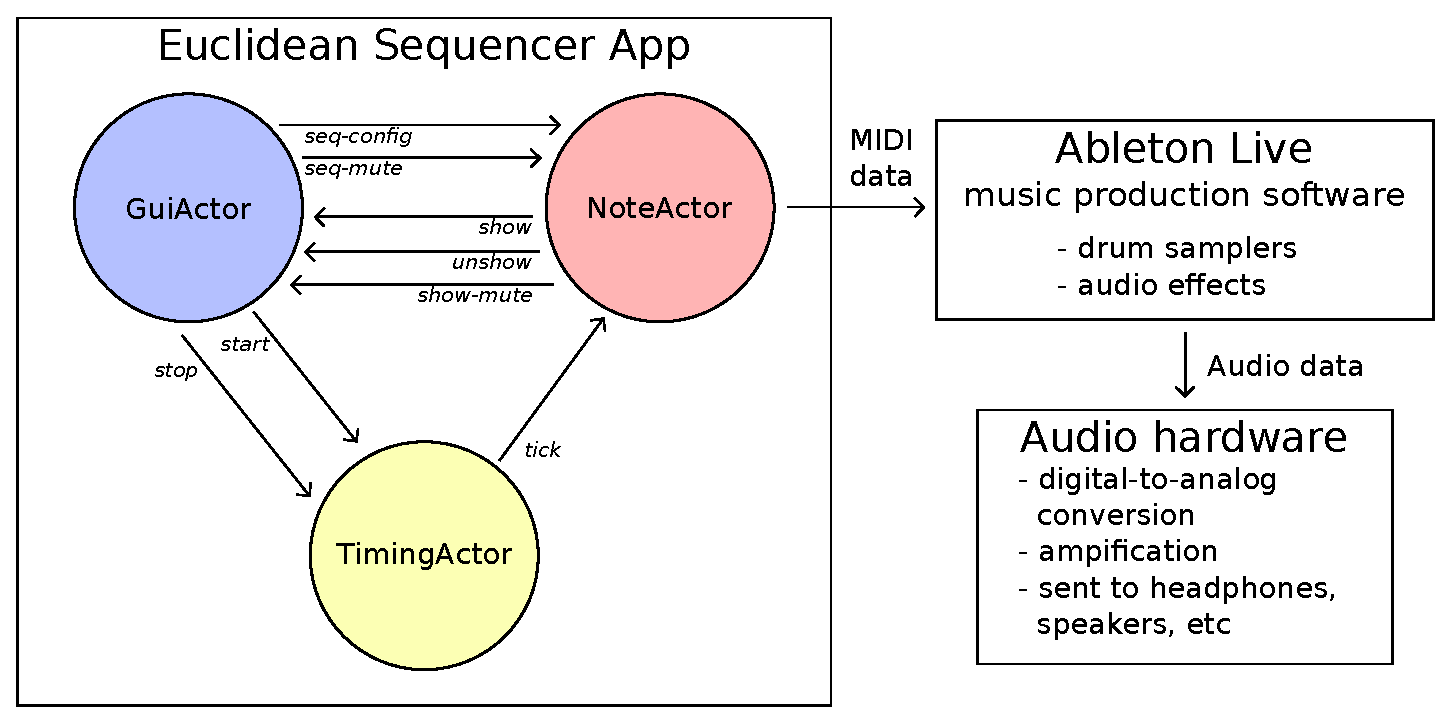
\includegraphics[width=\linewidth]{img/diagram.eps}
\caption{A block diagram that shows both the Actor structure used in
the Euclidean Sequencer application and the application's relationship
to the overall audio processing chain}
\label{block-diagram}
\end{figure}

\section{Conclusions}

The Euclidean rhythm sequencer application has been successfully implemented for interactive real-time performance. It has been shown that the Actor model of concurrency is well suited to solving the problem of musical synchronization by separating asynchronous user interaction, synchronous timing, and the application's logical state. The use of Python's generators has also been shown to be well suited to modeling Euclidean rhythms and other cyclic musical sequences.

To provide more extensive performance options, \textsc{midi} control of the application could be offered in order to allow for hardware control of the Euclidean rhythms instead of control by mouse and keyboard. 

%
% The following two commands are all you need in the
% initial runs of your .tex file to
% produce the bibliography for the citations in your paper.
\bibliographystyle{abbrv}
\bibliography{sigproc}  % sigproc.bib is the name of the Bibliography in this case

\end{document}
